\documentclass[border=10pt]{standalone}

\usepackage{tikz}
\usepackage{tikzsymbols}
\usetikzlibrary{calc,patterns,shapes.geometric}

\def\centerarc[#1](#2)(#3:#4:#5){\draw[#1] ($(#2)+({#5*cos(#3)},{#5*sin(#3)})$) arc (#3:#4:#5);}

\begin{document}
	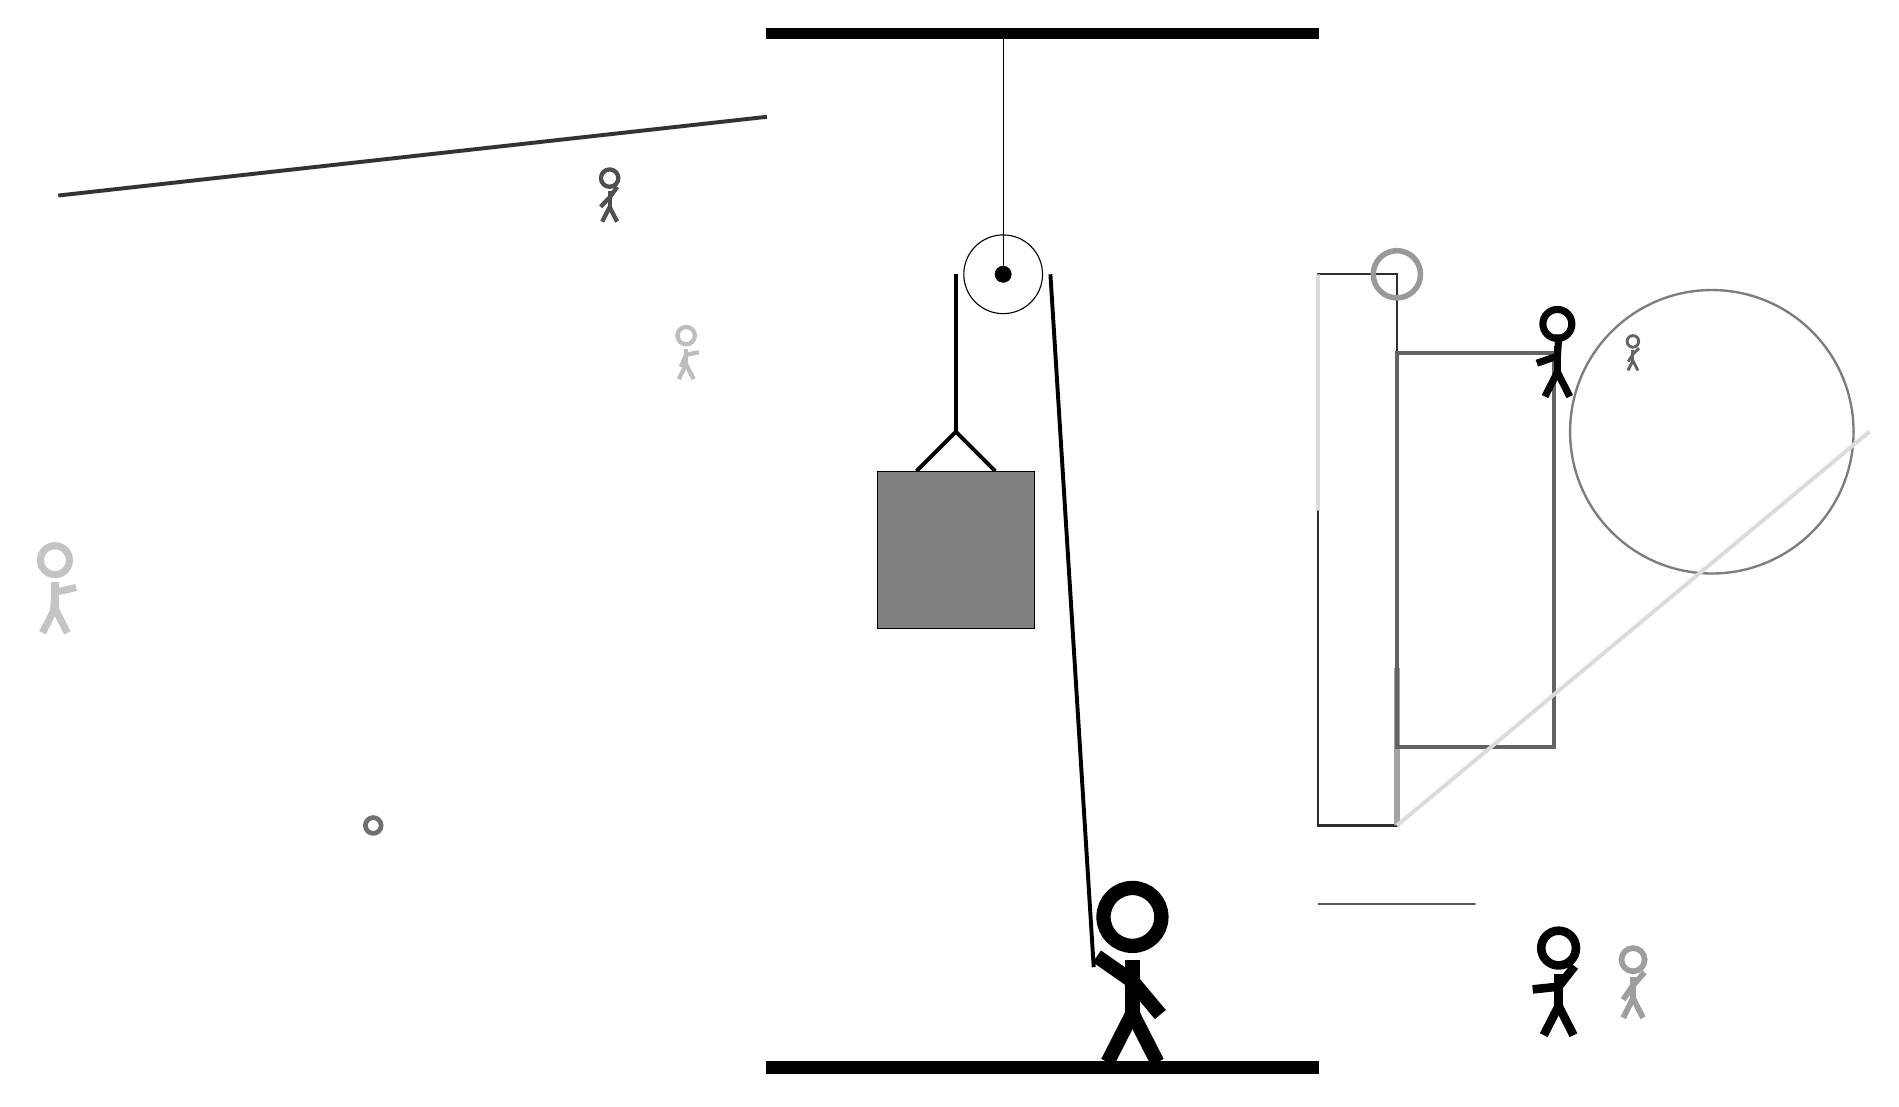
\begin{tikzpicture}
		%%%%% START %%%%%
		
		\draw[fill=black] (-2, 10) rectangle (5, 10.125);
		
		\draw (1, 7) circle (0.5);
		\draw[fill=black] (1, 7) circle (0.1);
		\draw (1, 10) -- (1, 7);
		
		\draw[line width=0.3mm, color=black!82] (5, 7) rectangle (6, 0);
		
		\node[line width=0.3mm, color=black!61] at (9, 6) {\Strichmaxerl[2][57][45]};
		\draw [line width=0.6mm, color=black!56](-7, 0) circle (0.1);
		\draw[line width=0.7mm, color=black!36] (6, 0) rectangle (6, 2);
		\node[line width=0.6mm, color=black!69] at (-4, 8) {\Strichmaxerl[3][46][54]};
		\node[line width=0.6mm, color=black!100] at (8, -2) {\Strichmaxerl[6][6][52]};
		\node[line width=0.2mm, color=black!23] at (-11, 3) {\Strichmaxerl[5][86][13]};
		\node[line width=0.3mm, color=black!38] at (9, -2) {\Strichmaxerl[4][55][49]};
		\draw[line width=0.5mm, color=black!80](-2, 9) -- (-11, 8);
		\draw[line width=0.3mm, color=black!66] (5, -1) rectangle (7, -1);
		\draw [line width=0.3mm, color=black!51](10, 5) circle (1.8);
		\draw[line width=0.5mm, color=black!61] (6, 6) rectangle (8, 1);
		\node[line width=0.2mm, color=black!98] at (8, 6) {\Strichmaxerl[5][19][86]};
		
		\node[line width=0.3mm, color=black!26] at (-3, 6) {\Strichmaxerl[3][66][12]};
		\draw [line width=0.7mm, color=black!40](6, 7) circle (0.3);
		\draw[line width=0.6mm, color=black!14] (5, 7) rectangle (5, 4);
		\draw[line width=0.5mm, color=black!14](6, 0) -- (12, 5);
		
		\draw[line width=0.5mm] (-0.1, 4.5) -- (0.4, 5.0) -- (0.9, 4.5);
		\draw[fill=black!50] (-0.6, 4.5) rectangle (1.4, 2.5);
		
		\draw[line width=0.5mm] (0.4, 7) -- (0.4, 5.0);
		\centerarc[line width=0.5mm](1, 7)(0:180:0.6);
		\draw[line width=0.5mm](1.6, 7) -- (2.15, -1.8);
		
		\node at (2.6, -1.9) {\Strichmaxerl[10][-35][-50]};
		
		\draw[fill=black] (-2, -3) rectangle (5, -3.15);
		
		%%%%% END %%%%%
	\end{tikzpicture}
\end{document}